The attack we implemented is aimed at intercepting HTTP cookies on a network the attacker has access to. In addition, cookies might have been set before the attack was actually started. Albeit it is required that either the cookie does not have the \emph{Secure} flag enabled or is send over an insecure connection during the attack.

A graphical representation of the attack can be seen in \autoref{fig:attack-scenario}. Below will the corresponding steps in the attack be elaborated:
\begin{enumerate}
	\item The victim connects to \texttt{S1} before the attack starts, and sets a cookie. Possibly using a secure connection.
\end{enumerate}

\noindent \emph{The attacker acquires a man-in-the-middle (MitM) position% between \texttt{Victim}, \texttt{S1} and \texttt{S2}
, for example using ARP poisoning.}
\begin{enumerate}
	\setcounter{enumi}{1}
	\item \texttt{Victim} requests a web page over HTTP to another server, since the attacker is in a MitM position will it instead be redirected to the attacker.
	\item \texttt{Attacker} redirects the request to the actual recipient in order to obtain a legitimate request.
	\item Again as a result of the MitM position will the response of the request be redirected back to the \texttt{Attacker}.
	\item The \texttt{Attacker} injects an image into the HTTP traffic with a reference to \texttt{S1} over an insecure connection.
	\item \texttt{Victim} tries to retrieve the image by sending an insecure request to \texttt{S1}, which contains the cookie set in~(1). This request is intercepted by the \texttt{Attacker} whom now has the desired cookie.
\end{enumerate}

\begin{figure}[t!]
	\centering
	\begin{subfigure}{0.4\textwidth}
	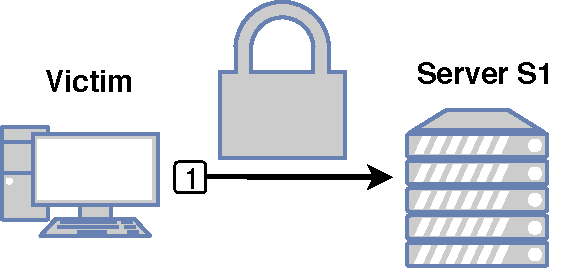
\includegraphics[width=\textwidth]{img/pre-attack}
		\caption{Before the attack.}
	\end{subfigure}

	\begin{subfigure}{0.4\textwidth}
		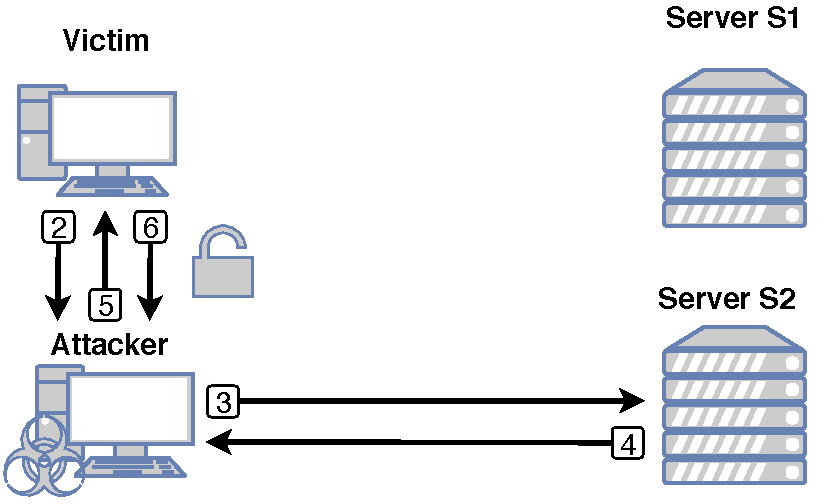
\includegraphics[width=\textwidth]{img/attack}
		\caption{During the attack.}
	\end{subfigure}
\caption{
	Graphical representation of the communication flow during the attack.}
	\label{fig:attack-scenario}
\end{figure}

An example use case of this attack could be that \texttt{S1} is the web server of an online banking service. The victim logged in earlies onto this service on a network which he or she actually trusts. Later on, the network changes and the victim does not trust the new environment enough and stops interacting with \texttt{S1}. Now the victim would expect that, without explicitly connecting to \texttt{S1}, his/her confidentiality with \texttt{S1} is untouched when interacting with other servers. Still does this attack manage to trick the victim into breaking the confidentiality, without raising any alert either by the victim or the banking service.
